\documentclass[12pt]{article}

\usepackage{vmargin}
\usepackage{setspace}
\usepackage[ruled, linesnumbered, french, onelanguage]{algorithm2e}
\usepackage{amsmath, amsthm, amssymb, amsfonts}
\usepackage{enumitem}
\usepackage[utf8]{inputenc}
\usepackage{hyperref}
\usepackage{graphicx}
\usepackage{float} % here for H placement parameter
\usepackage{qtree}
\usepackage{amsfonts}
\graphicspath{{figures/}}

\setlength{\parindent}{0pt}

\title{Devoir 2}
\author{Jérémy Bouchard}
\date{\today}


\begin{document}

\begin{titlepage}
	\doublespacing
	\centering

	UNIVERSITÉ DU QUÉBEC À CHICOUTIMI \\

	\vspace{4.7cm}

	DEVOIR 2 \\

	\vspace{4.7cm}

	PAR \\
	JÉRÉMY BOUCHARD (BOUJ08019605) \\
	JEAN-PHILIPPE SAVARD (SAVJ04079609) \\
	ALEXIS VALOTAIRE (VALA09129509) \\

	\vspace{4.7cm}

	DEVOIR PRÉSENTÉ À \\
	M. FRANÇOIS LEMIEUX \\
	DANS LE CADRE DU COURS D'ALGORITHMIQUE (8INF433)
\end{titlepage}

\newpage

\textit{Note :} Le code source \LaTeX \:est disponible à l'URL suivant : \\
\url{https://github.com/AlexisCode101/algo-devoir-2}

\newpage

\onehalfspacing

\section*{Question 1}
Le théorème sur les récurrences que nous avons vu en classe possède
une version plus simple dans le cas où la fonction f(n) est un polynôme.
Lorsque la récurrence est de la forme:
\begin{align*}
	T(n) = aT\Big(\frac{n}{b}\Big) + cn^k
\end{align*}

où c et k sont des constantes réelles positives, alors la solution est
donnée par:

\[T(n) \begin{cases}
      \Theta\big(n^{log_ba}\big) & \text{si } a>b^k \\
      \Theta\big(n^klg \: n\big) & \text{si } a=b^k \\
      \Theta\big(n^k\big) & \text{si } a<b^k
   \end{cases}
\]

Nous avons vu en classe la démonstration du premier cas (où  \(a > b^k\)
).
Utilisez le théorème sur les récurrences vu en classe pour démontrer les
deux autres cas.


\subsection*{Cas 2:}

Nous voulons démonter le cas où:
\begin{align*}
	a = b^k
\end{align*}

\noindent Pour ce faire, on commence par mettre le tout en
\(  log_b\), ce qui donne:
\begin{align*}
	 log_b(a) = log_b(b^k)
\end{align*}

Nous savons aussi qu'un log en base `X` de `X` équivaut à 1, donc:
\begin{align*}
	 log_b(a) = k
\end{align*}

Donc, on peut dire que:
\begin{align*}
	 n^k = n^{log_b(a)}
\end{align*}

Ainsi, nous satisfaisons la condition du cas 2 du théorème de récurrence, qui est:
\begin{align*}
	f(n) = \Theta\big(n^{log_b(a)} \: \big)
\end{align*}

Donc, par le fait même, on peut dire que:
\begin{align*}
	T(n) = \Theta\big(n^{log_b(a)} \: lg \: n \: \big) = \Theta\big(n^k \: lg \: n \: \big)
\end{align*}


\subsection*{Cas 3:}

Pour ce cas, nous avons deux conditions à satisfaire:
    \begin{enumerate}[label=(\alph*)]
      \item  il existe \( \epsilon > 0 \) tel que \( f(n) = \Omega\big(n^{log_ba+\epsilon}  \big) \)
      \item il existe \( c < 1 \) tel que \(af(n/b) \leq cf(n) \)
    \end{enumerate}


\subsubsection*{Condition a:}

Comme dans le cas 2, nous pouvons dire:
\begin{align*}
	a < b^k =  log_b(a) <  k
\end{align*}

Nous pouvons aussi dire que:
\begin{align*}
	log_b(a) <  k = 0 < -log_b(a) + k
\end{align*}

On peut alors supposer que:
\begin{align*}
	\epsilon = -log_b(a) + k
\end{align*}

Si on isole la valeur `K`, nous obtenons:
\begin{align*}
	k = log_b(a) + \epsilon
\end{align*}

Nous pouvons alors dire que:
\begin{align*}
	n^k = n ^{log_b(a) + \epsilon}
\end{align*}

Ainsi, nous respectons la première condition qui dit qu'il existe \( \epsilon > 0 \) tel que \( f(n) = \Omega\big(n^{log_ba+\epsilon}  \big) \)


\subsubsection*{Condition b:}
En divisant toute l'équivalence par \(b^k\), nous obtenons:
\begin{align*}
	a < b^k =  \frac{a}{b^k} < 1
\end{align*}

Nous pouvons alors supposer que:
\begin{align*}
	c =  \frac{a}{b^k}
\end{align*}

Ainsi, nous respection  la deuxième condition qui dit qu'il existe  \( c < 1 \) tel que \( af(n/b) \leq cf(n) \)


\newpage

\section*{Question 2}
L’algorithme de Dijkstra que nous avons vu en classe, nous permet
d’obtenir la longueur du plus court chemin entre un noeud source et
tous les autres noeuds mais il ne donne pas les chemins eux-mêmes. Comment modifieriez-vous cet algorithme afin d’obtenir cette information? Notez que la modification est mineure si vous choisissez la bonne façon de représenter les chemins. \newline

Il est possible de modifier l'algorithme de Djikstra facilement pour réaliser cela. En effet, nous n'avons qu'à tenir une liste des chemins vers chaque noeud à partir de noeud de départ. \newline

Nous n'avons qu'à modifier la valeur de ces chemins chaque fois que nous modifions la distance minimal dans l'algorithme. En effet, à chaque fois que nous modifions la distance minimale dans le tableau des distances de Djikstra, nous n'avons qu'à modifier les tableaux du chemin en la remplacant par la distance du noeud courant vers le noeud calculé. \newline

Prenons par exemple le graphe pour la question 3. Utilisons-le pour faire une démonstration, en supposant que celui-ci n'est pas orienté.

\begin{figure}[H]
	\centering
	\includegraphics[width=12cm]{figures/q3}
\end{figure}

Le tableau suivant montre les chemins entre le différents noeuds au début, en prenant le noeud 1 comme étant celui de départ.

\begin{center}
	\begin{tabular}{||c c||}
		\hline
		Noeud & Chemin \\ [0.5ex]
		\hline\hline
		1 & 1 \\
		\hline
		2 & - \\
		\hline
		3 & - \\
		\hline
		4 & - \\
		\hline
		5 & -  \\
		\hline
		6 & -  \\
		\hline
		7 & -  \\
		\hline
		8 & -  \\ [1ex]
		\hline
	\end{tabular}
\end{center}

Nous calculons ensuite le chemin vers les distances des noeuds adjacents à 1. La distance minimale a 2 doit être mise à jour, pusiqu'elle est présentemement infini, et qu'infini est plus petit que 8. On modifie donc le tableau pour que celui-ci ressemble à ceci.

\begin{center}
	\begin{tabular}{||c c||}
		\hline
		Noeud & Chemin \\ [0.5ex]
		\hline\hline
		1 & 1 \\
		\hline
		2 & 1-2 \\
		\hline
		3 & - \\
		\hline
		4 & - \\
		\hline
		5 & -  \\
		\hline
		6 & -  \\
		\hline
		7 & -  \\
		\hline
		8 & -  \\ [1ex]
		\hline
	\end{tabular}
\end{center}

De manière analogue, pour le noeud 3.

\begin{center}
	\begin{tabular}{||c c||}
		\hline
		Noeud & Chemin \\ [0.5ex]
		\hline\hline
		1 & 1 \\
		\hline
		2 & 1-2 \\
		\hline
		3 & 1-3 \\
		\hline
		4 & - \\
		\hline
		5 & -  \\
		\hline
		6 & -  \\
		\hline
		7 & -  \\
		\hline
		8 & -  \\ [1ex]
		\hline
	\end{tabular}
\end{center}

On se déplace ensuite au noeud 2 comme étant le noeud courant. En visitant ses noeuds adjacents, on voit que la distance vers le noeud 4 était infini. Pusiqu'il existe un lien qui nous permet de nous déplacer vers ce noeud à partir de 2, mettons le à jour. Ici, puisque nous sommes au noeud 2 comme noeud courant, le chemin vers 4 devient le chemin vers 2 plus le chemin de 4 à partir de 2. De manière analogue, nous obtenons aussi le chemin pour le noeud 5.

\begin{center}
	\begin{tabular}{||c c||}
		\hline
		Noeud & Chemin \\ [0.5ex]
		\hline\hline
		1 & 1 \\
		\hline
		2 & 1-2 \\
		\hline
		3 & 1-3 \\
		\hline
		4 & 1-2-4 \\
		\hline
		5 & 1-2-5  \\
		\hline
		6 & -  \\
		\hline
		7 & -  \\
		\hline
		8 & -  \\ [1ex]
		\hline
	\end{tabular}
\end{center}

Pour ce qui est du noeud 3, par contre, nous constatons que la distance entre du noeud de départ au noeud courant (2) plus la distance entre celui-ci et le noeud 3 est inférieure à celle dans le tableau de Djikstra. Il faut donc le mettre à jour. Le chemin vers le noeud 3 devient donc le chemin du noeud de départ vers le noeud courant plus le chemin du noeud cournat vers le noeud 3. Le tableau devient donc ceci.

\begin{center}
	\begin{tabular}{||c c||}
		\hline
		Noeud & Chemin \\ [0.5ex]
		\hline\hline
		1 & 1 \\
		\hline
		2 & 1-2 \\
		\hline
		3 & 1-2-3 \\
		\hline
		4 & 1-2-4 \\
		\hline
		5 & 1-2-5  \\
		\hline
		6 & -  \\
		\hline
		7 & -  \\
		\hline
		8 & -  \\ [1ex]
		\hline
	\end{tabular}
\end{center}

Il ne nous reste donc qu'à appliquer cet algorithme de Djikstra modifié pour obtenir le tableau des chemins, ce qui est une modification triviale de l'algorithme de Djikstra. En effet, nous n'avons qu'à construire un tableau analogue et le mettre à jour que lorsque un chemin est plsu petit, comme dans l'algorithme clasique de Djikstra.

\newpage

\section*{Question 3}
Considérez le graphe dirigé de la figure suivante:

\begin{figure}[H]
	\centering
	\includegraphics[width=12cm]{q3}
\end{figure}

Montrez le contenu du tableau \(D\), de l’ensemble \(S\) ainsi que la valeur de la variable \(v\) après chacune des itérations de l’algorithme. Décrivez toutes les étapes de l’algorithme Dijkstra. Utilisez le noeud 1 comme source. \\

\begin{table}[H]
\centering
\begin{tabular}{c|ccc}
Étape     & v & S                                  & D \\ \hline
    0     & - &  \(\lbrace 2,3,4,5,6,7,8 \rbrace\)   & \([8,10,\infty,\infty,\infty,\infty,\infty]\)  \\
    1     & 2 &  \(\lbrace 3,4,5,6,7,8 \rbrace\)     & \([8,9,16,18,\infty,\infty,\infty]\)  \\
    2     & 3 &  \(\lbrace 4,5,6,7,8 \rbrace\)       & \([8,9,16,18,\infty,\infty,\infty]\)  \\ 
    3     & 4 &  \(\lbrace 5,6,7,8 \rbrace\)         & \([8,9,16,17,24,26,\infty]\)  \\
    4     & 5 &  \(\lbrace 6,7,8 \rbrace\)           & \([8,9,16,17,24,26,\infty]\)  \\
    5     & 6 &  \(\lbrace 7,8 \rbrace\)   		     & \([8,9,16,17,24,25,32]\)  \\
    6     & 7 &  \(\lbrace 8 \rbrace\)   			 & \([8,9,16,17,24,25,32]\)  \\
\end{tabular}
\end{table}

\textbf{Étape 0 :} Seul la distance du noeud 1 aux noeuds 2 et 3 sont connus, les distances sont placées dans le tableau D. Le noeud 2 possède la distance la plus courte de D, v est donc égal au noeud 2. \\

\textbf{Étape 1 :} À l'aide du noeud 2, nous trouvons la distance entre le noeud 1 et les noeuds 4 et 5. Le noeud 3 possède la distance la plus courte de D en excluant les variables v précédentes, v est donc égal au noeud 3. \\

\textbf{Étape 2 :} Rien ne change dans le tableau D puisque les distances apportées par le noeud 3 sont plus grandes que ceux apportées par le noeud 2. Le noeud 4 possède la distance la plus courte de D en excluant les variables v précédentes, v est donc égal au noeud 4. \\

\textbf{Étape 3 :} À l'aide du noeud 4, nous trouvons un chemin plus court jusqu'au noeud 5 ainsi que les distances des noeuds 6 et 7. Le noeud 4 possède la distance la plus courte de D en excluant les variables v précédentes, v est donc égal au noeud 5. \\

\textbf{Étape 4 :} Rien ne change dans le tableau D puisque les distances apportées par le noeud 5 sont plus grandes que ceux apportées par le noeud 4. Le noeud 6 possède la distance la plus courte de D en excluant les variables v précédentes, v est donc égal au noeud 6. \\

\textbf{Étape 5 :} À l'aide du noeud 6, nous trouvons un chemin plus court jusqu'au noeud 7 ainsi que la distance jusqu'au noeud 8. Le noeud 7 possède la distance la plus courte de D en excluant les variables v précédentes, v est donc égal au noeud 7. \\

\textbf{Étape 6 :} Rien ne change dans le tableau D puisque les distances apportées par le noeud 7 sont plus grandes que ceux apportées par le noeud 6. L'algorithme s'arrête donc ici car toutes les plus courtes distances ont été trouvées. \\

\newpage

\section*{Question 4}
Résoudre les récurrences suivantes. \\

\textbf{a) } \(T(n)=2T\big(\frac{n}{2}\big)+1\) \\

\(a=2, \quad b=2, \quad n^{\log_ba} = n^{\log_22}=n \text{ et } f(n) = 1\) \\

Cas 1 : \(T(n) = \Theta(n^{\log_ba}) = \Theta(n^{\log_22}) = \Theta(n) \) \\

Car il existe un \(\epsilon>0\) tel que \(1 = O(n^{1-\epsilon}) \) par exemple \(\epsilon=0.9\) \\

\textbf{b) } \(T(n)=T\big(\frac{9n}{10}\big)+n\) \\

\(a=1, \quad b=\frac{10}{9}, \quad n^{\log_ba} = n^{\log_{\frac{10}{9}}1}=n^0=1 \text{ et } f(n) = n\) \\

Cas 3 : \(T(n)=\Theta(f(n))= \Theta(n) \) \\

(i) il existe un \(\epsilon>0\) tel que \(n = \Omega(n^{0+\epsilon}) \) par exemple \(\epsilon=1\) \\
(ii) il existe un \(c < 1\) tel que \( \frac{9n}{10} \leq cn \) par exemple \(c=\frac{9}{10}\) \\

\textbf{c) } \(T(n)=16T\big(\frac{n}{4}\big)+n^2\) \\

\(a=16, \quad b=4, \quad n^{\log_ba} = n^{\log_416}=n \text{ et } f(n) = n^2\) \\

Cas 2 : \(T(n) = \Theta(n^{\log_ba}lg \, n) = \Theta(n^{\log_416}lg \, n) = \Theta(n^2lg \, n) \) \\

Car \(n^2 = \Theta(n^2) \) \\

\textbf{d) } \(T(n)=7T\big(\frac{n}{3}\big)+n^2\) \\

\(a=7, \quad b=3, \quad n^{\log_ba} = n^{\log_37}=n^{1.77} \text{ et } f(n) = n^2\) \\

Cas 3 : \(T(n)=\Theta(f(n))= \Theta(n^2) \) \\

(i) il existe un \(\epsilon>0\) tel que \(n^2 = \Omega(n^{1.77+\epsilon}) \) par exemple \(\epsilon=0.22\) \\
(ii) il existe un \(c < 1\) tel que \( 7 \big(\frac{n}{3} \big)^2 \leq cn^2 \) par exemple \(c=\frac{7}{9}\) \\

\textbf{e) } \(T(n)=7T\big(\frac{n}{2}\big)+n^2\) \\

\(a=7, \quad b=2, \quad n^{\log_ba} = n^{\log_27}=n^{2.81} \text{ et } f(n) = n^2\) \\

Cas 1 : \(T(n) = \Theta(n^{\log_ba}) = \Theta(n^{\log_27}) = \Theta(n^{2.81}) \) \\

Car il existe un \(\epsilon>0\) tel que \(n^2 = O(n^{2.81-\epsilon}) \) par exemple 0 \\

\textbf{f) } \(T(n)=2T\big(\frac{n}{4}\big)+\sqrt{n}\) \\

\(a=2, \quad b=4, \quad n^{\log_ba} = n^{\log_42}=n^{\frac{1}{2}} \text{ et } f(n) = n^{\frac{1}{2}}\) \\

Cas 2 : \(T(n) = \Theta(n^{\log_ba}lg \, n) = \Theta(n^{\log_42}lg \, n) = \Theta(n^{\frac{1}{2}}lg \, n) \) \\

Car \(n^{\frac{1}{2}} = \Theta(n^{\frac{1}{2}}) \) \\

\textbf{g) } \(T(n)=3T\big(\frac{n}{2}\big)+5n\) \\

\(a=3, \quad b=2, \quad n^{\log_ba} = n^{\log_23}=n^{1.58} \text{ et } f(n) = 5n\) \\

Cas 1 : \(T(n) = \Theta(n^{\log_ba}) = \Theta(n^{\log_23}) = \Theta(n^{1.58}) \) \\

Car il existe un \(\epsilon>0\) tel que \(5n = O(n^{1.58-\epsilon}) \) par exemple 0.28 \\

\textbf{h) } \(T(n)=T\big(\frac{n}{2}+5\big)+1\) \\

Nous voyons que cette fois la formule est de la forme \(T(n) = aT \big(\frac{n}{b}+k \big) + f(n) \) \\

\(a=1, \quad b=2, \quad k=5 \quad et \quad f(n) = 1\) \\

Calculons \(c = \frac{kb}{b-1} = \frac{5*2}{2-1} = 10\) \\

Posons \(S(n) = T(n+c) = T(n+10) \) \\

Nous obtenons alors, 
\begin{align*}
	S(n) &= T(\frac{n+10}{2}+5)+1 \\
	&= T(\frac{n}{2}+10)+1 \\
	&= S(\frac{n}{2}) + 1
\end{align*}

Cas 2 : \(S(n) = \Theta(n^{\log_ba}lg \, n) = \Theta(n^{\log_21}lg \, n) = \Theta(lg \, n) \) \\
En ramenant en \(T(n)\) nous obtenons \(T(n)=\Theta(lg \, (n+10))\) \\

Car \(1 = \Theta(1)\) \\
\newpage

\section*{Question 5}
Considérez la matrice suivante
\begin{align*}
	F =
	\begin{pmatrix}
		0 & 1 \\
		1 & 1
	\end{pmatrix}
\end{align*}

Soit \(i\) et \(j\), deux entiers. Quel est le produit du vecteur (\(i\), \(j\)) et de la matrice \(F\)? Qu’arrive-t-il si i et j sont deux nombres consécutifs de la suite de Fibonacci? Utilisez cette idée pour concevoir un algorithme diviser-pour-régner capable de calculer le nième nombre de Fibonacci en temps \(\Theta (log \: n)\) en considérant (faussement) que les multiplications prennent un temps constant. Expliquez le lien entre votre algorithme et l’algorithme fib3 du devoir 1. \newline

Il est possible de constater que le résultat de la multiplication suivante :
\begin{align*}
	\begin{pmatrix}
		f_{n-1} & f_{n-2}
	\end{pmatrix}
	\cdot
	\begin{pmatrix}
		0 & 1 \\
		1 & 1
	\end{pmatrix}
	=
	\begin{pmatrix}
		f_{n-1} & f_{n-1} + f_{n-2}
	\end{pmatrix}
\end{align*}

Il est possible de se rapeller l'identité de la séquence de Fibbonaci :
\[ f_{n} = f_{n-1} + f_{n-2} \]

Il est donc possible de remplacer une identité dans la première équation :
\begin{align*}
	\begin{pmatrix}
		f_{n-1} & f_{n-2}
	\end{pmatrix}
	\cdot
	\begin{pmatrix}
		0 & 1 \\
		1 & 1
	\end{pmatrix}
	=
	\begin{pmatrix}
		f_{n-1} & f_{n}
	\end{pmatrix}
\end{align*}

On remarque qu'on peut chaîner la multiplication de la matrice. On observe que l'indice de la séquence de Fibonacci augmente à chaque itération. On peut observer cela grâce aux équations suivantes.
\begin{align*}
	\begin{pmatrix}
		f_{0} & f_{1}
	\end{pmatrix}
	\cdot
	\begin{pmatrix}
		0 & 1 \\
		1 & 1
	\end{pmatrix}
	=
	\begin{pmatrix}
		f_{0} & f_{0} + f_{1}
	\end{pmatrix}
\end{align*}

\begin{align*}
	\begin{pmatrix}
		f_{1} & f_{2}
	\end{pmatrix}
	\cdot
	\begin{pmatrix}
		0 & 1 \\
		1 & 1
	\end{pmatrix}
	=
	\begin{pmatrix}
		f_{1} & f_{1} + f_{2}
	\end{pmatrix}
\end{align*}

En chaînant les multiplications par la matrice, on constate la relation suivante.
\begin{align*}
	\begin{pmatrix}
		f_{0} & f_{1}
	\end{pmatrix}
	\cdot
	\begin{pmatrix}
		0 & 1 \\
		1 & 1
	\end{pmatrix}
	^n
	=
	\begin{pmatrix}
		f_{n} & f_{n+1}
	\end{pmatrix}
\end{align*}

En remplacant \( f_{0} \) et \( f_{1} \) par leurs valeurs respectives.
\begin{align*}
	\begin{pmatrix}
		0 & 1
	\end{pmatrix}
	\cdot
	\begin{pmatrix}
		0 & 1 \\
		1 & 1
	\end{pmatrix}
	^n
	=
	\begin{pmatrix}
		f_{n} & f_{n+1}
	\end{pmatrix}
\end{align*}

On observe également par multiplication successive de la matrice, les valeurs suivantes.
\begin{align*}
	\begin{pmatrix}
		0 & 1 \\
		1 & 1
	\end{pmatrix}
	^n
	=
	\begin{pmatrix}
		f_{n-1} & f_{n} \\
		f_{n} & f_{n+1}
	\end{pmatrix}
\end{align*}


Il ne reste donc qu'à calculer la matrice à la bonne puissance pour obtenir les valeurs de la séquence de Fibonacci. Il ne reste qu'à prouver que l'exponentiation d'une matrice peut se faire en \(\Theta (log \: n)\). \newline

Il est possible de calculer l'exponentiation de la matrice en multipliant les matrices dont l'exposant est divisé en 2 récursivement de la manière suivante. \newline

\Tree[.M^n [.M^{n/2} [.M^{n/4} [.$\cdots$ [.M^2 M^1 M^1 ]
										 											[.M^2 M^1 M^1 ]]]
               			 [.M^{n/4} [.$\cdots$ [.M^2 M^1 M^1 ]
																					[.M^2 M^1 M^1 ]]]]
        	 [.M^{n/2} [.M^{n/4} [.$\cdots$ [.M^2 M^1 M^1 ]
																					[.M^2 M^1 M^1 ]]]
                		 [.M^{n/4} [.$\cdots$ [.M^2 M^1 M^1 ]
																					[.M^2 M^1 M^1 ]]]]] \newline

 Il est donc possible de voir que l'on divise le problème à chaque étage. La hauteur de l'arbre est donc de \( log_2 (n) \). pusique l'on divise le problème à chaque itération. Puisqu'il faut multiplier la matrice par elle même \( log_2 (n) \) fois et que chaque multiplication ce fait en \(\Theta (1) \), l'algorithme se résoud en \(\Theta (log \: n)\). \newline

Cet algorithme assume que les valeurs de l'exposant soit d'un multiple de 2. Par contre, il est possible d'exprimer n'importe quel nombre comme étant une addition de plusieurs multiples de 2. Cela est possible de la manière suivante.

\[ n = \sum_{p \in P_n}^{} 2^p \]
\[ p \subset \mathbb{N}_0 \]

On comprend donc que l'exponentiation de la matrice est la suivante.

\[ M^n = \prod_{p \in P_n}^{} M^{2^p} \]
\[ p \subset \mathbb{N}_0 \]

Pour ce qui est du lien avec fib3 du devoir 1, il s'agit exactement de cet algorithme. Dans le devoir 1, l'algorithme effectuait des itérations en divisant le \( n \) par 2 à chaque itération et en calculant la multiplication de la matrice. La fonction fib3 est donc l'implémentation de cet algorithme.

\newpage

\section*{Question 6}
Soit \(X[1 \dots n]\) et \(Y [1 \dots n]\) deux tableaux, chacun contenant \(n\) nombres déjà triés. Donnez un algorithme diviser-pour-régner pour trouver le médian des \(2n\) éléments présents dans les tableaux \(X\) et \(Y\). Le temps d’exécution de votre algorithme doit être dans \(\Theta (log \: n)\) en pire cas.

\begin{flushleft}
L'algorithme suivant trouve la médiane de deux tableaux de même taille (taille `n`) de nombres triés. Il est à noter que la fonction `Mediane` utilisée aux lignes 7 et 8 est une fonction qui s'exécute en temps constant qui retourne la médiane d'un tableau.
\end{flushleft}


\begin{algorithm}[H]
      \KwData{\( X[1 \cdot\cdot\cdot  n], Y[1 \cdot\cdot\cdot  n], entier \: n \)}
      \KwResult{réel med}
      	\If{ \(n = 1\)}{
      		\Return \(  \big( \frac{X[1] + Y[1]}{2} \big) \) \
      	}

      	\If{ \(n = 2\)}{
      		\Return \(  \big( \frac{ max(X[1], Y[1]) + min(X[2], Y[2])   }{2} \big) \) \
      	}

      	\(medX \gets Mediane(X[1 \cdot\cdot\cdot  n]) \) \;
      	\(medY \gets Mediane(Y[1 \cdot\cdot\cdot  n]) \) \;

      	\If{\(medX = medY\)}{
      		\Return medX
      	}

      	\eIf{\(medX < medY\)}
      	{
      		\eIf{\( n\bmod  2 = 0\)}
      		{
      			\Return TrouverMédiane(X[\( \frac{n}{2} +1\) ...  n], Y[1 ...  \( \frac{n}{2} -1\)], \( \frac{n}{2} +1\))
      		}
      		{
      			\Return TrouverMédiane(X[\( \frac{n}{2}\) ...  n], Y[1 ...  \( \frac{n}{2}\)], \( \frac{n}{2}\))
      		}
      	}
      	{
      		      		\eIf{\( n\bmod  2 = 0\)}
      		{
      			\Return TrouverMédiane(X[1 ...  \( \frac{n}{2} -1\)], Y[\( \frac{n}{2} +1\) ...  n], \( \frac{n}{2} +1\))
      		}
      		{
      			\Return TrouverMédiane(X[\( \frac{n}{2}\) ...  n], Y[1 ...  \( \frac{n}{2}\)], \( \frac{n}{2}\))
      		}
      	}


      \caption{TrouverMédiane}
\end{algorithm}

\end{document}
